\documentclass[10pt]{article}

% Change "review" to "final" to generate the final (sometimes called camera-ready) version.
% Change to "preprint" to generate a non-anonymous version with page numbers.
\usepackage{acl}

% Standard package includes
\usepackage{times}
\usepackage{latexsym}
\usepackage{amsmath}
\usepackage{booktabs}
\usepackage{amssymb}
% For proper rendering and hyphenation of words containing Latin characters (including in bib files)
\usepackage[T1]{fontenc}
% For Vietnamese characters
% \usepackage[T5]{fontenc}
% See https://www.latex-project.org/help/documentation/encguide.pdf for other character sets

% This assumes your files are encoded as UTF8
\usepackage[utf8]{inputenc}

% This is not strictly necessary, and may be commented out,
% but it will improve the layout of the manuscript,
% and will typically save some space.
\usepackage{microtype}

% This is also not strictly necessary, and may be commented out.
% However, it will improve the aesthetics of text in
% the typewriter font.
\usepackage{inconsolata}

%Including images in your LaTeX document requires adding
%additional package(s)
\usepackage{graphicx}

% Tighter lists, floats, captions and equations
\usepackage{enumitem}
\setlist{nosep}
\setlist[description]{nosep, leftmargin=1.4em, labelindent=0pt}
\setlength{\textfloatsep}{8pt plus 2pt minus 2pt}
\setlength{\floatsep}{6pt plus 2pt minus 2pt}
\setlength{\intextsep}{6pt plus 2pt minus 2pt}
\setlength{\dbltextfloatsep}{8pt plus 2pt minus 2pt}
\setlength{\dblfloatsep}{6pt plus 2pt minus 2pt}
\setlength{\abovecaptionskip}{4pt}
\setlength{\belowcaptionskip}{0pt}
\makeatletter
\g@addto@macro\normalsize{%
  \setlength{\abovedisplayskip}{4pt plus 2pt minus 2pt}%
  \setlength{\belowdisplayskip}{4pt plus 2pt minus 2pt}%
  \setlength{\abovedisplayshortskip}{2pt plus 1pt}%
  \setlength{\belowdisplayshortskip}{2pt plus 1pt}}
\makeatother
\raggedbottom  % no stretched gaps between paragraphs to fill each column
\makeatletter
\g@addto@macro\UrlBreaks{\do\-}  % long URLs may break after a hyphen
\makeatother

% If the title and author information does not fit in the area allocated, uncomment the following
%
%\setlength\titlebox{<dim>}
%
% and set <dim> to something 5cm or larger.

% added by Reinout
\usepackage{lipsum}

\title{Low-Bit Quantization for Multilingual Machine Translation}

% Author information can be set in various styles:
% For several authors from the same institution:
% \author{Author 1 \and ... \and Author n \\
%         Address line \\ ... \\ Address line}
% if the names do not fit well on one line use
%         Author 1 \\ {\bf Author 2} \\ ... \\ {\bf Author n} \\
% For authors from different institutions:
% \author{Author 1 \\ Address line \\  ... \\ Address line
%         \And  ... \And
%         Author n \\ Address line \\ ... \\ Address line}
% To start a separate ``row'' of authors use \AND, as in
% \author{Author 1 \\ Address line \\  ... \\ Address line
%         \AND
%         Author 2 \\ Address line \\ ... \\ Address line \And
%         Author 3 \\ Address line \\ ... \\ Address line}

\author{
  Krijn Dignum \quad Francesco Massafra \quad Matthijs Vork \quad
  Max Wilde \quad Reinout Wolting \\
  University of Amsterdam \\
  \small\texttt{\{UvAnetID, 16101499, UvAnetID, 13839837, 13998110\}}
}

%\author{
%  \textbf{First Author\textsuperscript{1}},
%  \textbf{Second Author\textsuperscript{1,2}},
%  \textbf{Third T. Author\textsuperscript{1}},
%  \textbf{Fourth Author\textsuperscript{1}},
%\\
%  \textbf{Fifth Author\textsuperscript{1,2}},
%  \textbf{Sixth Author\textsuperscript{1}},
%  \textbf{Seventh Author\textsuperscript{1}},
%  \textbf{Eighth Author \textsuperscript{1,2,3,4}},
%\\
%  \textbf{Ninth Author\textsuperscript{1}},
%  \textbf{Tenth Author\textsuperscript{1}},
%  \textbf{Eleventh E. Author\textsuperscript{1,2,3,4,5}},
%  \textbf{Twelfth Author\textsuperscript{1}},
%\\
%  \textbf{Thirteenth Author\textsuperscript{3}},
%  \textbf{Fourteenth F. Author\textsuperscript{2,4}},
%  \textbf{Fifteenth Author\textsuperscript{1}},
%  \textbf{Sixteenth Author\textsuperscript{1}},
%\\
%  \textbf{Seventeenth S. Author\textsuperscript{4,5}},
%  \textbf{Eighteenth Author\textsuperscript{3,4}},
%  \textbf{Nineteenth N. Author\textsuperscript{2,5}},
%  \textbf{Twentieth Author\textsuperscript{1}}
%\\
%\\
%  \textsuperscript{1}Affiliation 1,
%  \textsuperscript{2}Affiliation 2,
%  \textsuperscript{3}Affiliation 3,
%  \textsuperscript{4}Affiliation 4,
%  \textsuperscript{5}Affiliation 5
%\\
%  \small{
%    \textbf{Correspondence:} \href{mailto:email@domain}{email@domain}
%  }
%}
\setlength\titlebox{4cm}
\begin{document}
\maketitle

\section{Introduction}

Machine translation (MT) has traditionally relied on encoder--decoder
architectures \citep{sutskever2014seq2seq,bahdanau2015neural}, most notably the
Transformer \citep{vaswani2017attention}. Massively multilingual systems such as
NLLB-200 \citep{nllb2022} carry this paradigm to 200 languages and remain strong
reference points for translation quality. The success of decoder-only large
language models (LLMs) in language modelling \citep{brown2020gpt3,touvron2023llama2}
has since shifted attention towards using them as translators \citep{hendy2023gpt}.
ALMA \citep{xu2024alma} showed that a moderately sized LLM becomes a strong
translator after continued monolingual pre-training followed by fine-tuning on a
small amount of high-quality parallel data. Its successor, ALMA-R
\citep{xu2024cpo}, introduces Contrastive Preference Optimization (CPO), which
teaches the model to prefer better translations over adequate but flawed ones
instead of imitating human references. Built on LLaMA-2-13B and trained with only
22K parallel sentences, ALMA-13B-R matches or exceeds the WMT competition winners
and GPT-4 on the WMT'21 and WMT'22 test sets, across ten translation directions
between English and Czech, German, Icelandic, Chinese and Russian.

Although small by LLM standards, ALMA-13B-R occupies 26\,GB on disk and needs
more than 25\,GiB of GPU memory to run, beyond what consumer GPUs provide.
Post-training quantization \citep{frantar2023gptq} reduces this cost, but its
damage to translation is uneven across languages and largest for lower-resource
ones \citep{marchisio2024quantization}. We quantize ALMA-13B-R with GPTQ to 8, 4,
3 and 2 bits. Then, keeping the quantizer fixed, we train a small LoRA adapter
\citep{hu2022lora} on the two most degraded models by knowledge distillation
from the full-precision model \citep{hinton2015distilling}. 

We address three research questions:

\begin{description}
  \item[RQ1] How do memory, speed and translation quality change as precision
             decreases from 16 to 2 bits, and is the loss uniform across
             languages?
  \item[RQ2] Can a distilled adapter recover the translation quality of the
             3-bit and 2-bit models without changing the quantizer?
  \item[RQ3] Which errors remain once the 2-bit model is recovered?
\end{description}

We evaluate on the WMT'22 test sets (WMT'21 for Icelandic), following the ALMA-R
protocol. Besides BLEU and chrF++ \citep{papineni2002bleu,popovic2017chrf}, we
use the reference-based COMET-22 \citep{rei2022comet22} and MetricX-24
\citep{juraska2024metricx}, and the reference-free CometKiwi-22, KIWI-XXL and
XCOMET-XXL \citep{rei2022cometkiwi,rei2023scaling,guerreiro2024xcomet}, together
with teacher-forced likelihood, segment-level failure modes and the on-disk size,
peak GPU memory and latency of each model. We find that quantization reduces memory but not latency, that
quality collapses below 4 bits (Icelandic first), and that a distilled adapter
of under 0.5\,GiB restores the 3-bit model to full-precision quality and
recovers most of the translation quality of the 2-bit model, which then runs in under 6\,GiB.

\section{Method}

\subsection{Model and Data}

\paragraph{Model.} We use ALMA-13B-R \citep{xu2024cpo}, a 13B-parameter
decoder-only model built on LLaMA-2-13B \citep{touvron2023llama2}. Its training
has three stages. First, ALMA \citep{xu2024alma} continues pre-training on 12B
tokens of monolingual OSCAR text, to strengthen the model in the non-English
languages. Second, it fine-tunes a LoRA adapter \citep{hu2022lora} on a small set
of human-written parallel data. Third, ALMA-R replaces this supervised objective
with CPO: a further LoRA adapter is trained on triplets of candidate translations
ranked by quality-estimation metrics, so that the model learns to prefer the best
translation rather than imitate the reference. The released model has the
adapters merged into the weights. We prompt it in ALMA's format and decode with
beam search (beam size 5). Our full-precision reproduction matches the scores
reported by \citet{xu2024cpo}: averaged into and out of English, it is within
0.4 BLEU and 0.5 XCOMET-XXL, and within 1.1 points on every reported metric.

\paragraph{Data.} We cover the ten ALMA-R directions: English to and from Czech,
German, Icelandic, Russian and Chinese. We test on the WMT'22 test sets
\citep{kocmi2022findings}, and on WMT'21 for Icelandic
\citep{akhbardeh2021findings}, with 1{,}000--2{,}037 sentences per direction
(17{,}471 in total). For GPTQ calibration and adapter distillation, we use only
ALMA's human-written parallel training data (58.7K sentence pairs from earlier
WMT test sets and FLORES-200), which does not overlap with the test sets.

\subsection{Quantization Setup}
\paragraph{Method.} We use GPTQ \citep{frantar2023gptq}, a one-shot, weight-only
post-training quantization method. For each linear layer with weights
$\mathbf{W}$ and calibration inputs $\mathbf{X}$, GPTQ finds quantized weights
$\widehat{\mathbf{W}}$ that preserve the layer output:
\begin{equation}
  \widehat{\mathbf{W}} = \arg\min_{\widehat{\mathbf{W}}}
  \big\lVert \mathbf{W}\mathbf{X} - \widehat{\mathbf{W}}\mathbf{X} \big\rVert_2^2 .
\end{equation}
It quantizes the weights one column at a time and adjusts the remaining columns
to compensate for the rounding error, using second-order information from
$\mathbf{X}$ \citep{frantar2022obc}.

\paragraph{Configuration.} We quantize with the GPTQModel library
\citep{gptqmodel} at 8, 4, 3 and 2 bits, with identical settings for each
bit-width: asymmetric quantization with groups of 128 weights (each group stores
its own scale and zero-point), act-order (columns processed in order of
decreasing activation magnitude), and 1{,}024 calibration sentences
($\sim$105K tokens) from ALMA's training data, balanced over the ten directions.
All linear layers of the 40 decoder blocks are quantized (12.6B of the 13.0B
parameters). The embeddings, the output head and the normalization layers stay
in half precision.



\subsection{Post-Quantization Adaptation}
To recover the 3-bit and 2-bit models, we keep the quantized weights frozen and
add a LoRA adapter \citep{hu2022lora} to every linear layer, as in QLoRA
\citep{dettmers2023qlora}. Each quantized layer $\widehat{\mathbf{W}}$ becomes
\begin{equation}
  \mathbf{h} = \widehat{\mathbf{W}}\mathbf{x} + \tfrac{\alpha}{r}\,\mathbf{B}\mathbf{A}\mathbf{x},
\end{equation}
where only the low-rank matrices $\mathbf{A}$ and $\mathbf{B}$ (rank $r$) are
trained. The quantizer itself is never changed.

A natural choice would be to fine-tune the adapter on reference translations.
However, ALMA-R's advantage comes from CPO, which teaches the model to
\emph{outperform} the references rather than imitate them \citep{xu2024cpo}, and
supervised training on references would pull the model back towards them.
Instead, we use the full-precision model as a teacher and distil its behaviour
into the quantized student \citep{hinton2015distilling,kim2016sequence}. The
adapter minimises the Kullback--Leibler divergence
\citep{kullback1951information} between the teacher's and the student's
next-token distributions, over the target tokens of each translation:
\begin{equation}
  \mathcal{L} = \sum_{t}
  \mathrm{KL}\big( p_{\text{fp16}}(\cdot \mid \mathbf{x}, y_{<t})
  \,\|\, p_{\text{quant}}(\cdot \mid \mathbf{x}, y_{<t}) \big).
\end{equation}
Because the targets are the teacher's full distributions and not the references,
the student learns to reproduce the CPO-tuned model itself. We train on
examples from ALMA's parallel training data: 30K for the 3-bit model, with rank
$r=16$ (0.12\,GiB), and 90K for the 2-bit model, with rank $r=64$ (0.47\,GiB).


\subsection{Evaluation Metrics}
We follow the evaluation of ALMA-R \citep{xu2024cpo} and extend it. We report
two lexical metrics, BLEU \citep{papineni2002bleu} and chrF++
\citep{popovic2017chrf}, computed with sacreBLEU \citep{post2018sacrebleu}. Since
lexical overlap with a single reference can penalise valid translations, we also
use learned neural metrics. COMET-22 \citep{rei2022comet22} and MetricX-24
\citep{juraska2024metricx} compare the output with the reference. XCOMET-XXL
\citep{guerreiro2024xcomet}, CometKiwi-22 \citep{rei2022cometkiwi} and
KIWI-XXL \citep{rei2023scaling} are run reference-free, as in ALMA-R, so that
they judge a translation from its source alone and do not favour a reference
that the model may outperform. XCOMET-XXL is our primary metric. Differences are
tested with paired bootstrap resampling (1{,}000 samples, 95\% confidence
intervals).

To locate where quantization damages the model, independently of decoding, we
also measure teacher-forced negative log-likelihood (NLL) on the test sets. For
each direction, we compute the per-token NLL of the reference translation given
ALMA's prompt, with the loss on the target tokens only (\emph{translation NLL}).
For each language, we compute the per-token NLL of 500 test sentences on their
own, with no prompt (\emph{monolingual NLL}). We report the increase over the
full-precision model, $\Delta\mathrm{NLL} = \mathrm{NLL}_{\text{quant}} -
\mathrm{NLL}_{\text{fp16}}$, in nats per token. The first measures the
translation mapping and the second measures knowledge of the language itself.

Corpus-level averages can hide a small number of severe failures. For the
recovered 2-bit model, we therefore also analyse the tail of the distribution.
First, we count the share of failed translations (XCOMET-XXL $<0.5$) and the
critical error spans that XCOMET-XXL marks. Second, we flag four known NMT failure
modes at segment level: \emph{oscillation}, i.e.\ repetition loops detected by
top n-gram count \citep{raunak2021curious,guerreiro2023hallucinations};
\emph{off-target} output in the wrong language \citep{zhang2020improving},
detected with the NLLB language identifier \citep{nllb2022,joulin2017bag};
\emph{source copy} \citep{ott2018analyzing}; and \emph{under-translation}
\citep{tu2016modeling}, i.e.\ outputs shorter than half the reference.



\section{Results}

\subsection{Effect of Quantization on Translation Quality}

\begin{table}[h]
\centering
\footnotesize
\setlength{\tabcolsep}{1.6pt}
\begin{tabular}{lrrrrrrr}
\toprule
 & \multicolumn{3}{c}{Memory (GiB)} & Time & \multicolumn{3}{c}{Quality} \\
\cmidrule(lr){2-4}\cmidrule(lr){5-5}\cmidrule(lr){6-8}
 & & \multicolumn{2}{c}{Peak} & s/sent. & & & \\
Model & Disk & $b{=}1$ & $b{=}4$ &  & BLEU & XCOMET & MetricX \\
\midrule
fp16 & 24.2 & 25.4 & 28.8 & 0.36 & 31.4 & 92.1 & 2.38 \\
w8   & 12.7 & 13.9 & 17.2 & 0.60 & 31.4 & 92.1 & 2.38 \\
w4   &  6.8 &  8.9 & 12.3 & 0.46 & 30.5 & 91.3 & 2.48 \\
w3   &  5.3 &  6.8 & 10.1 & 1.19 & 23.3 & 78.4 & 4.72 \\
w2   &  3.8 &  5.0 & 11.7 & 4.71 &  0.0 & 22.7 & 9.91 \\
\midrule
w3+KD & 5.4 & 6.9 & 10.3 & 1.20 & 31.1 & 91.9 & 2.43 \\
w2+KD & 4.2 & 5.5 &  9.2 & 0.91 & 27.8 & 88.1 & 3.16 \\
\bottomrule
\end{tabular}
\caption{Memory and translation quality of ALMA-13B-R under GPTQ, without and
with the distilled adapter (KD). \emph{Peak}: peak GPU memory when translating
de$\rightarrow$en with beam 5 at batch size $b$, adapters in bf16.
\emph{Time}: s/sentence at $b{=}4$ on one H100. Both use packed weights (App.~\ref{app:training}).
Quality is averaged over the ten directions; XCOMET is XCOMET-XXL and MetricX is
MetricX-24 (lower is better).}
\label{tab:main}
\end{table}

Table~\ref{tab:main} reports the memory cost and the average quality of each
model. Down to 4 bits, quantization costs almost no quality. The 8-bit model
matches full precision on every metric: in no direction does XCOMET-XXL change
by more than 0.2 points. The 4-bit model loses 0.9 BLEU and 0.8 XCOMET-XXL on
average, and at most 1.3 XCOMET-XXL points in any direction, while its checkpoint
is $3.6\times$ smaller (24.2 to 6.8\,GiB). Peak GPU memory falls less than the
checkpoint size (28.8 to 12.3\,GiB), because activations and the key--value
cache are not quantized. This memory saving does not buy speed: on our
inference stack, no quantized model translates faster than the full-precision
model (Table~\ref{tab:main}). The 4-bit model, the only one with a fused kernel,
is the fastest quantized model at 0.46\,s per sentence against 0.36\,s for full
precision; the 3-bit model takes 1.19\,s, and the 2-bit model 4.71\,s, partly
because its degenerate outputs are much longer. The freed memory can still buy
throughput through larger batches: from batch size 4 to 16, the 3-bit model
becomes $2.8\times$ faster per sentence, against $1.6\times$ for full
precision. Full precision stays faster at equal batch size, but at batch size 16
it needs 42.3\,GiB, while the 3-bit model needs 23.3\,GiB.

\subsection{The Low-Bit Performance Cliff}

\begin{figure}[t]
\centering
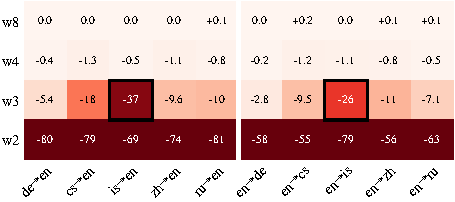
\includegraphics[width=\columnwidth]{figures/rq1_xcomet_delta.pdf}
\caption{Change in XCOMET-XXL relative to full precision, per direction and
bit-width. The colour scale saturates at $-40$. Boxed: Icelandic at 3 bits.}
\label{fig:rq1}
\end{figure}

Below 4 bits, quality drops sharply. At 3 bits, the average XCOMET-XXL falls
from 92.1 to 78.4 and MetricX-24 doubles. Figure~\ref{fig:rq1} shows that this
loss is far from uniform across languages. German is barely affected ($-5.4$ and
$-2.8$ XCOMET-XXL into and out of English), whereas Icelandic loses 37.4 and
25.8 points, about half of its BLEU in both directions. Icelandic is also the
language with the least parallel data in ALMA's training set and by far the rarest language covered (2K sentence pairs,
against 12--15K for the other languages), which agrees with the observation
that quantization hurts lower-resource languages most
\citep{marchisio2024quantization}. All seven quality metrics show the same
pattern (Appendix~\ref{app:full}, Table~\ref{tab:full}).

Simpler explanations do not hold. Calibration is not the cause: Icelandic
already has the largest share of the calibration tokens (22.2\%), and its
activations are no more outlier-heavy than German's. Nor are the Icelandic test
sentences simply harder: when sentences are matched by how confident the
full-precision model is, Icelandic's extra loss relative to the other
directions is unchanged (22.7 against 22.9 XCOMET-XXL points), and Icelandic is
the most damaged direction in every difficulty quintile. Finally, quantization
does not erase ALMA-R's translation fine-tuning: the fine-tuning update
survives almost exactly at every bit-width (Appendix~\ref{app:analyses}).

Teacher-forced likelihood shows what the 3-bit model loses for Icelandic
(Figure~\ref{fig:nll} in Appendix~\ref{app:full}). Its
monolingual NLL rises by 0.49 nats per token, in the middle of the range of the
other languages (0.22 for Chinese to 0.83 for Czech). The model therefore loses
no more of Icelandic itself than of the other languages. Its translation NLL,
however, rises more than for any other language in both directions (0.64 for
is$\rightarrow$en and 0.58 for en$\rightarrow$is, against at most 0.42
elsewhere). The model still models Icelandic text but has lost much of the
mapping between Icelandic and English.\footnote{Per-token NLL depends on how each
language is tokenized, so we compare languages by rank rather than by absolute
value.}

At 2 bits, the model collapses in every direction: BLEU falls to 0.0 and
XCOMET-XXL to 22.7. Between 97\% and 100\% of the outputs in each direction
show at least one failure mode: 62--96\% contain repetition loops and 79--100\%
are in the wrong language.
The collapse even raises peak memory above that of the 3-bit model (11.7
against 10.1\,GiB, Table~\ref{tab:main}), although the 2-bit weights are
smaller, because the degenerate outputs are much longer and fill the key--value
cache.

\subsection{Recovery Through Adapter Distillation}
\label{sec:recovery}

The likelihood analysis suggests that the 3-bit model keeps its knowledge of the
languages but loses the translation mapping, which is exactly what distillation
on translation data targets. The 2-bit model is damaged more broadly: its NLL
rises by 2.9--4.8 nats per token even on monolingual text. We therefore give it a
four times larger adapter ($r=64$ instead of 16) and a longer training run
(Appendix~\ref{app:training}).

\begin{figure}[t]
\centering
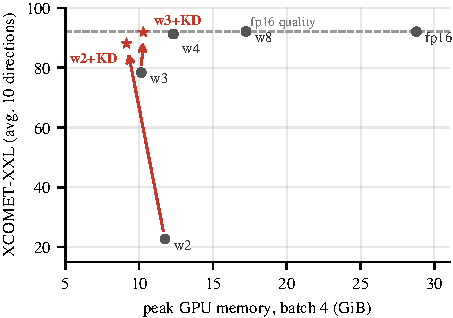
\includegraphics[width=\columnwidth]{figures/rq2_tradeoff.pdf}
\caption{Peak GPU memory (batch 4, adapters counted in bf16) against average
XCOMET-XXL. Arrows: the effect of the distilled adapter on the 3- and 2-bit
models.}
\label{fig:rq2}
\end{figure}

At 3 bits, the 0.12\,GiB adapter recovers 93--100\% of the increase in
translation NLL in every direction, and 96\% of the BLEU and 99\% of the
XCOMET-XXL loss on average (Table~\ref{tab:main}). In the 20 direction--metric
comparisons (ten directions, BLEU and XCOMET-XXL, paired bootstrap with 1{,}000
resamples), the recovered model is statistically indistinguishable from full
precision in 16. It is significantly better than the 4-bit model in 12 and
never worse, while being 1.4\,GiB smaller (Figure~\ref{fig:rq2}).

At 2 bits, the adapter turns a collapsed model into a usable translator. Average
BLEU rises from 0.0 to 27.8 and XCOMET-XXL from 22.7 to 88.1, which recovers
89\% and 94\% of the gap to full precision (Table~\ref{tab:main}). The
recovered 2-bit model scores higher than the plain 3-bit model on every metric,
significantly so in 18 of the 20 direction--metric comparisons and never lower,
although it is 1.1\,GiB smaller on disk, and at batch size 1 it needs 5.5\,GiB
of GPU memory, so, like the recovered 3-bit model (6.9\,GiB), it fits an
8\,GB consumer GPU.\footnote{With the adapter
counted in bf16. All runs keep the adapter in fp32 (5.9\,GiB measured); the
effect of bf16 rounding on quality was not measured.} The recovery is not
complete, however. Translation NLL recovers 96--99\% of the damage, but
monolingual NLL only 69--77\%: the adapter, trained only on translation,
restores the translation mapping much more than the language model itself.
Section~\ref{sec:tail} analyses the errors that remain.


\subsection{What Remains After Recovery}
\label{sec:tail}

\begin{table}[t]
\centering
\footnotesize
\setlength{\tabcolsep}{1.6pt}
\begin{tabular}{lrrrrrrrrrr}
\toprule
 & \multicolumn{5}{c}{into English} & \multicolumn{5}{c}{out of English} \\
\cmidrule(lr){2-6}\cmidrule(lr){7-11}
 & de & cs & is & zh & ru & de & cs & is & zh & ru \\
\midrule
fp16   & 0.5 & 0.6 & 0.2 & 3.1 & 1.7 & 0.5 & 1.3 & 0.1 & 1.3 & 1.7 \\
w3     & 0.7 & 0.8 & 3.5 & 6.8 & 2.1 & 0.5 & 3.1 & 14.7 & 7.0 & 3.3 \\
w2     & 97 & 100 & 100 & 97 & 100 & 100 & 100 & 100 & 100 & 100 \\
\midrule
w3+KD  & 0.5 & 0.5 & 0.3 & 3.0 & 1.7 & 0.4 & 1.2 & 0.1 & 1.5 & 1.2 \\
w2+KD  & 0.5 & 0.6 & 0.2 & 3.3 & 1.7 & \textbf{2.4} & 1.5 & \textbf{1.2} & \textbf{4.2} & 1.9 \\
\bottomrule
\end{tabular}
\caption{Share of outputs (\%) with at least one failure: oscillation,
off-target language, source copy, empty or under-translated output. Language
identification alone flags 0--1.8\% of the references. Bold: clearly above full
precision.}
\label{tab:failures}
\end{table}

Corpus-level averages could hide a model that games the metrics, for example by
producing fluent text that does not translate the source. Table~\ref{tab:failures}
shows that this is not the case. The plain 2-bit model fails on 97--100\% of the
segments, the recovered one on 0.2--4.2\%. In seven of ten directions, the
recovered 2-bit model stays within 0.3 percentage points of full precision, and
in nine of ten it fails less often than the plain 3-bit model, which is
1.1\,GiB larger. The recovered 3-bit model stays within 0.2 points of full
precision in every direction.

The remaining failures of the 2-bit model are concentrated in three directions
out of English, each with its own cause.\footnote{For Chinese targets, the
language identifier mislabels a quarter of the references, so we count an output
as off-target when fewer than half of its letters are Han characters. Our
oscillation flag uses the top n-gram count only, without the additional
low-quality condition of \citet{guerreiro2023hallucinations}.} In
en$\rightarrow$zh (4.2\%) and en$\rightarrow$is (1.2\%), they are mostly
repetition loops (2.75\% and 1.10\%, against 0.29\% and 0.10\% at full
precision). In en$\rightarrow$de (2.4\%), they are mostly source copies (1.77\%,
against none at full precision), almost all short interface strings such as
\textit{``Tap Settings.''}, which the model leaves in English.

Beyond these outright failures, the recovered 2-bit model translates somewhat
worse. XCOMET-XXL marks more critical errors than for full precision (e.g.\ 415
against 320 in is$\rightarrow$en, 211 against 123 in en$\rightarrow$zh), and more
translations score below 0.5 (17.4\% against 13.5\% in is$\rightarrow$en, 4.6\%
against 1.2\% in en$\rightarrow$is). The gap grows with sentence length: in
en$\rightarrow$is, the XCOMET-XXL difference to full precision widens from
$-3.6$ on the shortest quarter of the sources to $-12.4$ on the longest, and
en$\rightarrow$zh, is$\rightarrow$en and en$\rightarrow$cs follow the same trend.
These new errors are also not the ones full precision makes: only 12\% of the
2-bit model's worst 5\% of en$\rightarrow$is translations are among the worst 5\%
of full precision. Together with the partial recovery of monolingual likelihood
(Section~\ref{sec:recovery}), this suggests that the residual errors come from a
weaker language model, which hurts most when the model generates long text in a
lower-resource language.

\section{Conclusion}

Model compression is an invaluable resource in an era of ever larger models.
Strikingly large models achieve astonishing performance, but how to deploy them
outside the lab remains an open question. We show that ALMA-13B-R, a
state-of-the-art translation model that needs more than 25\,GiB of GPU memory,
can be compressed to 2 bits and, with a 0.47\,GiB distilled adapter, translate
in 5.5\,GiB, recovering 89--94\% of the quality that quantization destroyed. This puts high-quality machine
translation within reach of an 8\,GB consumer GPU, on the user's own machine.

Along the way, we find that quantization down to 4 bits is nearly free, and
that below it quality collapses unevenly, Icelandic first. The 3-bit model does
not forget Icelandic; it forgets how to translate it. A small adapter distilled
from the full-precision model restores this mapping: the 3-bit model returns to
full-precision quality, and the 2-bit model goes from unusable to a reliable
translator whose remaining errors are rare and well characterised.

Perhaps the most surprising result concerns the memory budget itself. Once
distillation is available, memory is better spent on an adapter than on bits.
The recovered 2-bit model (4.2\,GiB) outperforms the plain 3-bit model
(5.3\,GiB) on every metric, and the recovered 3-bit model (5.4\,GiB) matches
the 4-bit model (6.8\,GiB). Half a gigabyte of distilled parameters is worth
more than a whole extra bit per weight.

\section*{Limitations and Future Work}

\paragraph{Memory, not speed.} The memory savings of quantization do not
translate into faster inference in our setup. Only the 4-bit checkpoints have a
fused kernel; at the other bit-widths, the weights are dequantized to 16-bit
precision at every forward pass, so translation becomes slower as the bit-width
decreases (the 3-bit model is $3.3\times$ slower per sentence than full
precision). This is a kernel limitation, not an inherent cost: storing the same
3-bit values losslessly in the 4-bit layout already makes 3-bit generation
2.3--2.6$\times$ faster, at the cost of the larger 4-bit layout in memory
(Appendix~\ref{app:training}). Fused low-bit kernels would be needed for low-bit
models to be fast as well as small.

\paragraph{Incomplete recovery at 2 bits.} Distillation recovers the translation
mapping almost fully, but not the language model: monolingual likelihood
recovers only 69--77\% of the 2-bit damage. The recovered model still produces
language-dependent failures, such as repetition loops into Chinese and
Icelandic and untranslated English strings into German, and its quality drops
on long sentences.

\paragraph{Ablations we could not run.} Our design choices were made a priori
and not ablated, mainly for computational reasons. First, we chose distillation
over supervised fine-tuning on the references, motivated by CPO; comparing the
two would show whether this choice holds empirically. Second, we raised the
adapter rank from 16 to 64 for the 2-bit model, expecting rank 16 to lack the
capacity to repair a model damaged everywhere. Since the bit-width and the rank
change together, a 2-bit run at rank 16 is needed to separate their effects.
Third, each result comes from a single training run and seed.

\paragraph{Scope of the evaluation.} The adapter is trained on all ten test
directions, so we do not know whether it repairs the model in general or only
the directions it saw. Training without Icelandic and testing on it, or testing
on languages ALMA never saw, would answer this. Our evaluation relies on
automatic metrics only; XCOMET-XXL and KIWI-XXL were also used to build ALMA-R's
preference data, which may favour ALMA-R and its distilled copies, a risk we
mitigate with the independent MetricX-24 but do not remove. Finally, memory was
measured on a data-centre GPU; the 8\,GB claim assumes a recent NVIDIA GPU with
bf16 support and has not been tested on consumer hardware. Older GPUs could in
principle run the model in fp16 or fp32, at a much lower speed.

\section*{Code Availability}

Our code is available under the MIT licence at
\url{https://github.com/krijnD/-Model-Compression-for-Machine-Translation-in-Large-Language-Models/tree/francesco/refactor-public}.
It covers the full pipeline: the reproduction of ALMA-13B-R, GPTQ quantization,
adapter distillation, evaluation and all analyses, with the exact command of
every run reported here. The repository also contains the scores and
measurements behind every result, and the scripts that rebuild all figures and
tables of this paper from them. The quantized checkpoints and the distilled
adapters can be rebuilt with these scripts.

% Bibliography entries for the entire Anthology, followed by custom entries
%\bibliography{custom,anthology-overleaf-1,anthology-overleaf-2}

% Custom bibliography entries only
\bibliography{custom}

\newpage

\appendix

\section{Additional Results}
\label{app:full}

Table~\ref{tab:full} gives the score of every model on every metric and
direction.

% Generated by scripts/paper/make_full_table.py, do not edit by hand.
\begin{table*}[t]
\centering
\footnotesize
\setlength{\tabcolsep}{4.2pt}
\begin{tabular}{lrrrrrrrrrrrrr}
\toprule
 & de$\rightarrow$en & cs$\rightarrow$en & is$\rightarrow$en & zh$\rightarrow$en & ru$\rightarrow$en & Avg & en$\rightarrow$de & en$\rightarrow$cs & en$\rightarrow$is & en$\rightarrow$zh & en$\rightarrow$ru & Avg & All \\
\midrule
\multicolumn{14}{l}{\textit{BLEU} ($\uparrow$)} \\
fp16 & 31.6 & 44.8 & 40.2 & 22.9 & 39.6 & 35.8 & 28.1 & 26.2 & 22.3 & 33.9 & 24.4 & 27.0 & 31.4 \\
w8 & 31.6 & 44.9 & 40.0 & 23.0 & 39.6 & 35.8 & 28.0 & 26.5 & 22.3 & 33.8 & 24.2 & 27.0 & 31.4 \\
w4 & 31.2 & 43.9 & 39.1 & 22.5 & 39.5 & 35.2 & 27.0 & 24.8 & 21.8 & 31.6 & 23.4 & 25.7 & 30.5 \\
w3 & 29.1 & 32.1 & 20.2 & 15.2 & 31.5 & 25.6 & 25.2 & 21.6 & 12.1 & 25.3 & 20.4 & 20.9 & 23.3 \\
w2 & 0.1 & 0.0 & 0.0 & 0.1 & 0.0 & 0.0 & 0.0 & 0.1 & 0.0 & 0.0 & 0.0 & 0.0 & 0.0 \\
w3+KD & 31.4 & 43.9 & 39.8 & 22.6 & 39.8 & 35.5 & 28.0 & 25.9 & 22.1 & 33.1 & 24.3 & 26.7 & 31.1 \\
w2+KD & 30.0 & 41.1 & 35.9 & 19.7 & 36.4 & 32.6 & 25.7 & 22.6 & 17.4 & 28.0 & 21.4 & 23.0 & 27.8 \\
\midrule
\multicolumn{14}{l}{\textit{chrF++} ($\uparrow$)} \\
fp16 & 55.3 & 67.3 & 61.7 & 52.2 & 64.2 & 60.1 & 55.7 & 52.2 & 50.6 & 28.4 & 50.1 & 47.4 & 53.8 \\
w8 & 55.3 & 67.3 & 61.7 & 52.3 & 64.2 & 60.2 & 55.6 & 52.4 & 50.6 & 28.2 & 50.0 & 47.4 & 53.8 \\
w4 & 55.0 & 66.5 & 61.1 & 51.8 & 64.2 & 59.7 & 55.0 & 51.6 & 50.3 & 27.5 & 49.7 & 46.8 & 53.3 \\
w3 & 52.8 & 56.7 & 43.1 & 42.8 & 58.1 & 50.7 & 52.5 & 47.6 & 38.5 & 22.0 & 45.5 & 41.2 & 46.0 \\
w2 & 4.7 & 3.5 & 4.4 & 3.8 & 3.4 & 4.0 & 6.5 & 4.7 & 5.1 & 0.4 & 0.5 & 3.4 & 3.7 \\
w3+KD & 55.1 & 66.7 & 61.1 & 51.9 & 64.1 & 59.8 & 55.4 & 52.1 & 50.1 & 27.7 & 50.1 & 47.1 & 53.4 \\
w2+KD & 53.7 & 64.1 & 57.6 & 48.5 & 61.3 & 57.1 & 52.5 & 48.5 & 45.6 & 24.5 & 46.8 & 43.6 & 50.3 \\
\midrule
\multicolumn{14}{l}{\textit{COMET-22} ($\uparrow$)} \\
fp16 & 85.0 & 87.0 & 87.3 & 81.6 & 85.6 & 85.3 & 86.9 & 90.6 & 87.0 & 87.0 & 88.8 & 88.1 & 86.7 \\
w8 & 85.0 & 87.0 & 87.2 & 81.6 & 85.6 & 85.3 & 86.8 & 90.6 & 87.0 & 87.0 & 88.7 & 88.0 & 86.7 \\
w4 & 84.8 & 86.7 & 86.8 & 81.1 & 85.3 & 84.9 & 86.5 & 90.3 & 86.8 & 86.5 & 88.5 & 87.7 & 86.3 \\
w3 & 82.3 & 80.8 & 73.1 & 75.2 & 80.6 & 78.4 & 84.1 & 86.3 & 74.0 & 81.2 & 84.5 & 82.0 & 80.2 \\
w2 & 26.5 & 23.8 & 23.6 & 24.9 & 22.9 & 24.4 & 34.2 & 34.1 & 20.9 & 33.9 & 25.5 & 29.7 & 27.0 \\
w3+KD & 85.1 & 86.8 & 87.0 & 81.5 & 85.6 & 85.2 & 86.8 & 90.6 & 86.8 & 86.9 & 88.8 & 88.0 & 86.6 \\
w2+KD & 84.0 & 85.6 & 84.9 & 79.7 & 84.2 & 83.7 & 84.8 & 88.7 & 83.9 & 84.4 & 86.8 & 85.7 & 84.7 \\
\midrule
\multicolumn{14}{l}{\textit{MetricX-24} ($\downarrow$)} \\
fp16 & 2.95 & 3.70 & 3.36 & 1.66 & 2.75 & 2.88 & 0.69 & 2.73 & 3.26 & 1.29 & 1.39 & 1.87 & 2.38 \\
w8 & 2.94 & 3.70 & 3.36 & 1.66 & 2.75 & 2.88 & 0.69 & 2.72 & 3.29 & 1.30 & 1.38 & 1.88 & 2.38 \\
w4 & 3.04 & 3.80 & 3.45 & 1.92 & 2.87 & 3.02 & 0.74 & 2.82 & 3.38 & 1.40 & 1.42 & 1.95 & 2.48 \\
w3 & 4.06 & 5.92 & 8.39 & 3.97 & 4.36 & 5.34 & 1.31 & 4.58 & 9.06 & 2.68 & 2.84 & 4.09 & 4.72 \\
w2 & 7.99 & 11.68 & 10.04 & 7.70 & 9.68 & 9.42 & 8.23 & 12.90 & 12.85 & 7.70 & 10.33 & 10.40 & 9.91 \\
w3+KD & 2.97 & 3.74 & 3.41 & 1.76 & 2.78 & 2.93 & 0.73 & 2.79 & 3.40 & 1.33 & 1.41 & 1.93 & 2.43 \\
w2+KD & 3.37 & 4.20 & 4.20 & 2.39 & 3.28 & 3.49 & 1.18 & 3.73 & 5.22 & 1.96 & 2.09 & 2.84 & 3.16 \\
\midrule
\multicolumn{14}{l}{\textit{CometKiwi-22} ($\uparrow$)} \\
fp16 & 81.7 & 82.8 & 81.7 & 79.5 & 81.9 & 81.5 & 83.7 & 85.4 & 82.4 & 82.6 & 84.4 & 83.7 & 82.6 \\
w8 & 81.7 & 82.8 & 81.7 & 79.5 & 81.9 & 81.5 & 83.7 & 85.3 & 82.4 & 82.6 & 84.4 & 83.7 & 82.6 \\
w4 & 81.5 & 82.7 & 81.5 & 78.9 & 81.6 & 81.2 & 83.4 & 85.2 & 82.1 & 82.3 & 84.2 & 83.5 & 82.3 \\
w3 & 79.0 & 76.7 & 70.5 & 72.8 & 77.5 & 75.3 & 81.0 & 80.4 & 69.8 & 76.3 & 79.8 & 77.5 & 76.4 \\
w2 & 28.1 & 26.5 & 34.4 & 27.4 & 29.3 & 29.2 & 23.9 & 23.8 & 21.2 & 24.6 & 24.2 & 23.6 & 26.4 \\
w3+KD & 81.7 & 82.8 & 81.6 & 79.3 & 81.8 & 81.4 & 83.6 & 85.3 & 82.4 & 82.5 & 84.4 & 83.7 & 82.5 \\
w2+KD & 81.0 & 81.8 & 80.5 & 77.9 & 80.9 & 80.4 & 81.7 & 83.6 & 79.7 & 80.2 & 82.8 & 81.6 & 81.0 \\
\midrule
\multicolumn{14}{l}{\textit{KIWI-XXL} ($\uparrow$)} \\
fp16 & 84.5 & 84.2 & 86.0 & 77.4 & 81.7 & 82.7 & 85.3 & 88.7 & 86.4 & 85.2 & 88.3 & 86.8 & 84.8 \\
w8 & 84.5 & 84.3 & 86.0 & 77.5 & 81.7 & 82.8 & 85.3 & 88.7 & 86.3 & 85.1 & 88.4 & 86.8 & 84.8 \\
w4 & 84.0 & 83.6 & 85.5 & 76.5 & 81.2 & 82.2 & 84.5 & 87.5 & 85.6 & 84.3 & 87.5 & 85.9 & 84.0 \\
w3 & 77.7 & 68.3 & 58.1 & 64.3 & 72.1 & 68.1 & 77.8 & 75.2 & 56.3 & 70.6 & 76.0 & 71.2 & 69.6 \\
w2 & 0.3 & -1.4 & -1.0 & 2.2 & -0.9 & -0.1 & -2.1 & -1.3 & -3.7 & -1.6 & -1.9 & -2.1 & -1.1 \\
w3+KD & 84.2 & 83.7 & 85.9 & 77.2 & 81.7 & 82.5 & 84.9 & 88.3 & 86.0 & 84.8 & 88.0 & 86.4 & 84.5 \\
w2+KD & 81.9 & 80.1 & 82.2 & 73.1 & 79.1 & 79.3 & 79.5 & 80.7 & 76.0 & 77.9 & 82.1 & 79.2 & 79.3 \\
\midrule
\multicolumn{14}{l}{\textit{XCOMET-XXL} ($\uparrow$)} \\
fp16 & 94.7 & 88.7 & 81.2 & 91.8 & 91.5 & 89.6 & 97.7 & 94.4 & 92.8 & 92.5 & 95.4 & 94.6 & 92.1 \\
w8 & 94.6 & 88.8 & 81.1 & 91.8 & 91.7 & 89.6 & 97.7 & 94.6 & 92.8 & 92.6 & 95.5 & 94.6 & 92.1 \\
w4 & 94.2 & 87.4 & 80.7 & 90.7 & 90.8 & 88.8 & 97.5 & 93.2 & 91.7 & 91.6 & 94.9 & 93.8 & 91.3 \\
w3 & 89.2 & 70.3 & 43.8 & 82.2 & 81.3 & 73.3 & 95.0 & 84.9 & 67.0 & 81.6 & 88.3 & 83.4 & 78.4 \\
w2 & 14.7 & 9.7 & 12.6 & 17.5 & 10.7 & 13.0 & 39.3 & 39.9 & 13.5 & 36.0 & 32.6 & 32.3 & 22.7 \\
w3+KD & 94.5 & 88.4 & 81.2 & 91.7 & 91.4 & 89.4 & 97.5 & 93.9 & 92.8 & 92.3 & 95.3 & 94.4 & 91.9 \\
w2+KD & 92.7 & 84.1 & 76.5 & 88.8 & 89.0 & 86.2 & 95.8 & 89.2 & 85.3 & 86.8 & 92.3 & 89.9 & 88.1 \\
\bottomrule
\end{tabular}
\caption{Translation quality of every model in every direction, on WMT'22 (WMT'21 for Icelandic). \emph{Avg}: mean over the five directions into or out of English; \emph{All}: mean over all ten. XCOMET-XXL, CometKiwi-22 and KIWI-XXL are reference-free; the others use the reference.}
\label{tab:full}
\end{table*}


Figure~\ref{fig:nll} compares, at 3 bits, the loss in monolingual likelihood
with the loss in translation likelihood for each language.

\begin{figure}[h]
\centering
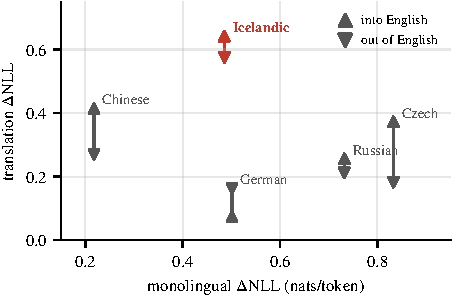
\includegraphics[width=\columnwidth]{figures/nll_w3.pdf}
\caption{Increase in teacher-forced NLL of the 3-bit model over full precision.
x-axis: monolingual text in each language; y-axis: reference translations into
($\blacktriangle$) and out of ($\blacktriangledown$) English. Icelandic loses
an average amount of the language but the most translation likelihood.}
\label{fig:nll}
\end{figure}

Figure~\ref{fig:adapter} compares the recovered 3-bit model with the 4-bit
model on the four directions scored first. The adapter closes gaps of up to 34.5
XCOMET-XXL points to within $\pm0.5$ of full precision, and it is closer to full
precision than the 4-bit model in 8 of 12 cells (3 tied, 1 worse), by a few
tenths of a point.
The difference to the 4-bit model is significant in 2 of 8 BLEU and XCOMET-XXL
comparisons (paired bootstrap): en$\rightarrow$is XCOMET-XXL ($+1.1$) and
en$\rightarrow$de BLEU ($+1.0$).

\begin{figure*}[t]
\centering
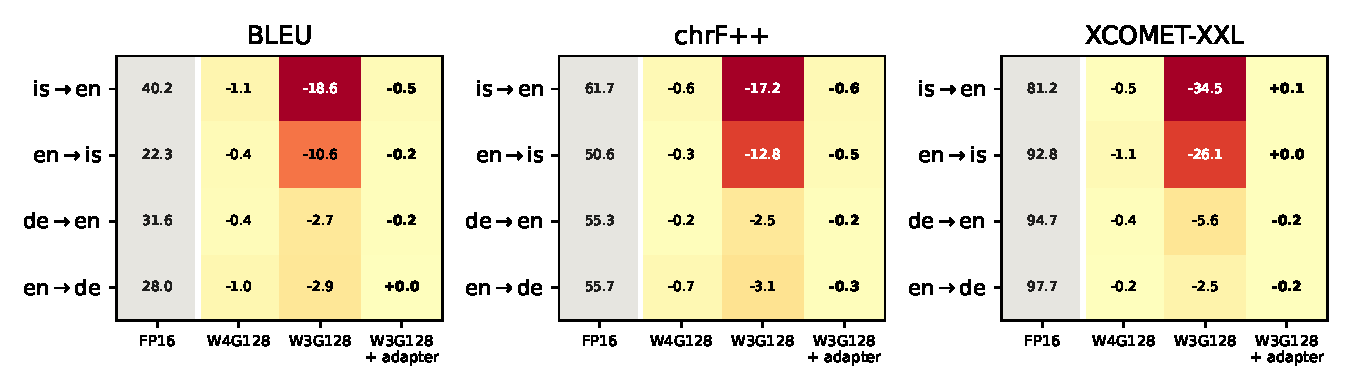
\includegraphics[width=\textwidth]{figures/w3_adapter_heatmap.pdf}
\caption{Difference to full precision (grey column: absolute fp16 scores) of
the 4-bit, plain 3-bit and recovered 3-bit models, on the four directions scored
first. Both 3-bit columns were generated on the repacked weights
(Appendix~\ref{app:training}), so they differ only by the adapter.}
\label{fig:adapter}
\end{figure*}

\section{Training Details}
\label{app:training}

\paragraph{Student and teacher.} The student is the GPTQ checkpoint with all
quantized weights frozen, plus a LoRA adapter on all seven linear layers
(query, key, value and output projections, and the three MLP projections) of all
40 decoder blocks. The teacher is the full-precision ALMA-13B-R.

\paragraph{Objective.} Token-level forward KL divergence from the teacher's to
the student's next-token distribution over the full vocabulary, computed on the
target tokens only. No loss is computed on the references.

\paragraph{Data.} 30K examples from ALMA's human-written parallel training data,
in ALMA's prompt format. Every Icelandic example appears twice ($2\times4{,}018$
over both directions), and the remaining examples are split evenly over the
other eight directions ($\sim$2{,}750 each). 32 sentence pairs per language pair
are held out to monitor the KL divergence. None of the data overlaps with the
test sets.

\paragraph{Hyperparameters.} AdamW, learning rate $2\cdot10^{-4}$ with 3\%
linear warm-up and cosine decay to 0, batch size 32 (16 $\times$ 2 gradient
accumulation steps), one epoch (936 steps), gradient checkpointing. LoRA scaling
$\alpha=2r$: $r=16$ for the 3-bit model (62.5M parameters) and $r=64$ for the
2-bit model (250M parameters). The 2-bit adapter is then trained for a second
run of 60K examples (1{,}873 steps) with a fresh learning-rate schedule, because
its held-out KL was still falling when the first schedule ended. Each run takes
40--80 minutes on one H100 (peak memory 36--37\,GiB).

\paragraph{Kernels and weight layout.} Training runs on the packed GPTQ weights
with a PyTorch kernel that supports backpropagation. All memory and latency
numbers (Table~\ref{tab:main}, Figure~\ref{fig:rq2}) are measured on the packed
checkpoints, with GPTQModel's default kernel for each bit-width (ExLlamaV2 for
4 bits, Triton for 8 and 2 bits, PyTorch for 3 bits), for the plain and the
recovered models alike. The translations of the plain models also come from the
packed checkpoints. Only the translations of the recovered models were generated
differently: to save GPU time, the 3- and 2-bit weights were repacked losslessly
into the 4-bit layout, which the faster ExLlamaV2 kernel accepts, and the
adapter was applied on top. The repacked weights are identical, but the kernel
computes in fp16 instead of bf16, so beam search can choose different outputs:
on the first 200 sentences, 80\% of the de$\rightarrow$en and 39\% of the
en$\rightarrow$is translations of the plain 3-bit model stay the same, and BLEU
changes by 0.2 and 0.4 points. Figure~\ref{fig:adapter} therefore compares the
recovered and the plain 3-bit model on the same repacked kernel. The 4-bit layout
also uses more memory: at batch size 4, the repacked 3-bit model peaks at
12.3\,GiB instead of 10.1\,GiB.

\section{Computational Requirements}
\label{app:compute}

All experiments ran on the Snellius national supercomputer, on nodes with
NVIDIA H100 (94\,GB) and A100 (40\,GB) GPUs, one GPU per job.

\paragraph{H100.} We ran on the H100 everything whose cost we compare across
models, so that run times are measured on identical hardware: the GPTQ
quantization (16.5 minutes per bit-width), the generation of all five
quantization levels (about 55 GPU-hours in total), and all latency
measurements. The H100 was also required, not just preferred, in two cases.
XCOMET-XXL and KIWI-XXL need about 43\,GB of memory, more than an A100 has, and
distillation training peaks at 36--37\,GiB, which nearly fills an A100 and runs
about three times slower on it. Each training run took 40--80 minutes, and
scoring one model on all ten directions with all metrics about 1.5 hours.

\paragraph{A100.} We moved to the A100 work whose result does not depend on the
GPU model. Peak-memory measurements are hardware-independent, so the batch-1
probes ran on the A100; we never compare run times across the two GPU types.

\section{Additional Analyses}
\label{app:analyses}

\paragraph{Quantization preserves the fine-tuning.} ALMA-13B-R is
ALMA-13B-Pretrain plus a merged LoRA adapter (supervised fine-tuning followed by
CPO), so the whole translation stage is a rank-16 update $\Delta$ to the MLP
down-projection of each block; all other weights are identical to the
pre-trained model. We compare $\Delta$ with the quantization error
$\widehat{\mathbf{W}}-\mathbf{W}$ in layers 0, 20 and 39. At 3 bits, the
rounding error is 4.5--9 times larger than $\Delta$ in Frobenius norm, and the
median entry of $\Delta$ is only 2--3\% of one quantization step. Rounding should
therefore wipe the update out, but it does not: the projection of the quantized
weights onto $\Delta$,
$\rho=\langle\widehat{\mathbf{W}}-\mathbf{W}_{\text{pre}},\Delta\rangle/\lVert\Delta\rVert^2$,
is 1.00--1.02 at every bit-width, because GPTQ rounds the fine-tuned weights, not
the pre-trained ones. The error is large but points elsewhere: at 3 bits, only
0.19--0.28\% of it lies in $\Delta$'s rank-16 subspace, exactly what isotropic
noise would give. The same quantities weighted by each language's activations
are equal across the five languages. The fine-tuning update thus survives
quantization equally for every language, which is why the damage shows up in the
model's outputs rather than as an erased fine-tuning stage.

\paragraph{Sanity checks of the 2-bit recovery.} We checked that the recovered
2-bit model translates rather than exploits the evaluation. (i) No test
sentence overlaps with the training data: no exact source or reference match,
and no shared 8-gram between a test source and the training file, in all ten
directions. (ii) It does not copy its teacher: its BLEU against the
full-precision outputs is 30--61 per direction, against 59--80 for the 4-bit
model, so it writes its own translations. (iii) It omits numbers from the source
no more often than full precision (e.g.\ 1.1\% against 1.3\% of the
is$\rightarrow$en segments). (iv) Before any XCOMET-XXL score of the first 2-bit
adapter existed, we fixed a success criterion of recovering at least 90\% of the
XCOMET-XXL gap in both is$\rightarrow$en and de$\rightarrow$en; that adapter
recovered 90.2\% and 96.8\%.

\end{document}
